\documentclass[10pt,a4paper]{article}
\usepackage[utf8]{inputenc}
\usepackage{amsmath}
\usepackage{amsfonts}
\usepackage{amssymb}
\usepackage{graphicx}
\author{Micky Faas}
\title{MIR - `ZoekMuis'}

\begin{document}
\maketitle

\section{Overview}

`ZoekMuis' is the name of my search-engine-lite project. I tried to do my best to ensure compatibility with the LIACS computers, but if something does not work, please let me know. It is also possible to download the entire project from GitHub:
\begin{verbatim}
https://github.com/mickymuis/zoekmuis
\end{verbatim}
\subsection{Components by others}

Some of the components used in this project were made by others. First of all, I have used the entire `imageretrieval' program and its libraries almost as-is. It can be found in the folder \texttt{imgcompare} and it is build to a separate executable. For the duplicate detection I have used an implementation of avl-trees taken from `zentut.com'. This implementation is far from perfect, but it makes the duplicate detection work at a decent speed. Moreover, I have picked Murmur2 as my main hashing function and DOCID. Its implementation was written by Austin Appleby. Last but not least I have also included  `htmlstreamparser' by Michael Kowalczyk.

\subsection{Features}

\begin{itemize}
\item Basic crawler and duplicate detection using avl-trees and hashing
\item Circular queue limits memory usage
\item Websearch using reverse indices for `link', `page', `web' and `title'
\item Image search using `alt' and page title
\item Weighted ranking
\item Color based image-matching
\end{itemize}

\subsection{Duplicate detection}

As far as duplicate URL detection is concerned, I have improved only slightly over the previous implementation. The previous implementation used a queue with a balanced binary tree (AVL) in conjunction with Murmur2 hashing (see below). This has proven work reasonably decent performance-wise, but the approach sometimes struggles with URLs that are the same, but are formulated differently. There is written alot about the subject of URL normalization, some of which is quite complex to implement. I have included at least a basic form of URL-sanitation (\texttt{docid\_sanitizeUrl()} to make the duplicate detection more accurate. 
\par The queue-with-avl implementation has kept the circular array as in the previous version as I decided against the use of a linked list. Both approaches have disadvantages (linked list used slightly more memory, wheres the circ. array relies on character-per-character comparisons). However, I believe the circular array to have superior locality over the linked list approach, though I have not tested this in any way. Perhaps more research can be done to find what datastructure would offer the greatest performance in this context (or just ask Google).

\subsection{Discussion}

Here I will discuss some of the limitations of the implementation and certain decisions I made that may be worthwhile mentioning. First of all, I have chosen to replace all URLs by DOCIDs instead. The Murmur2 hash used for DOCID is fast to generate and its 64 bit length prevents significant collisions, at least in this context. With this approach, the indices can be binary with fixed 8 byte fields, resulting in a significant reduction of memory footprint and lookup time. The downside is that reverse lookup (DOCID to URL) can be very expensive or needs a separate hashmap. Because of time constraints, I favoured an approach were I use the repository as reverse lookup. Instead of storing the complete HTML-page, every DOCID has an equally named file in \texttt{repository/} containing:
\begin{verbatim}
abs_url \n
page title \n
dump of HTML inner text elements
\end{verbatim}
For images, the two last fields are empty. One of the advantages is that the reverse lookup is now completely handled by the filesystem. The extraction of the HTML inner text proved to be hard using htmlstreamparser and is, in many cases, not very accurate or complete. This is definitely a point for improvement.\par
I have also decided to include image similarity queries based on color histograms. To this end I have modified the `imageretrieval' demo to output a list of DOCIDs instead of an HTML page. Because I did not want to mix my C and C++ code, I have kept the result as a separate executable (\texttt{imgcompare}) that is invoked by \texttt{webquery} if such a query is given. With more time, \texttt{imgcompare} could be made into a shared library to achieve some speedup and robustness.\par
Another limitation is the way the ranklist is generated. Currently, an associative array is employed and C's \texttt{qsort()} is used to sort it. However, the datastructure relies on exhaustive search to update its entries which will be extremely slow for larger indices. This could be alleviated by augmenting it with the already existing avl-tree or by turning it in a proper hashmap.\par
The last limitation worth to mention is the fact that currently only single-word queries are supported. Logical OR could be easily implemented, but the more usefull AND would obviously need to have at least some degree of preprocessing done on the indices. Luckily, the DOCID based incides make this already easy.

\subsection{Results and screenshots}

Results in terms of speed were generally very positive until I implemented the retrieval of \emph{all} images. Some pages, with many images, can take up to minutes to process (mind you, this is from my internet connection at home). The following statistics were obtained by lifting the domain restriction and crawling from \texttt{www.leiden.edu}:
\begin{itemize}
\item Total pages retrieved: 1240
\item Queue: in queue 30316, total size 2.45 Mb
\item Database: 637 Mb, from which 625 Mb for images
\item Total time: 71 minutes
\end{itemize} 
Second trail run with slightly updated code (bug fixes), starting from \texttt{http://leidenuniv.nl}:
\begin{itemize}
\item Total pages retrieved: 2000
\item Queue: in queue 41338, total size 2.6 Mb
\item Database: 753 Mb, from which 730 Mb for images
\item Total time: 121 minutes
\end{itemize} 
Unfortunately, `find by color' was too slow on this dataset to be usefull.
\newpage
Example of a webquery \newline

\includegraphics[width=12cm]{zoekmuis_web.png}\newline
Example of an image query \newline

\includegraphics[width=12cm]{zoekmuis_images.png}\newline
\newpage
Example of a color query\newline
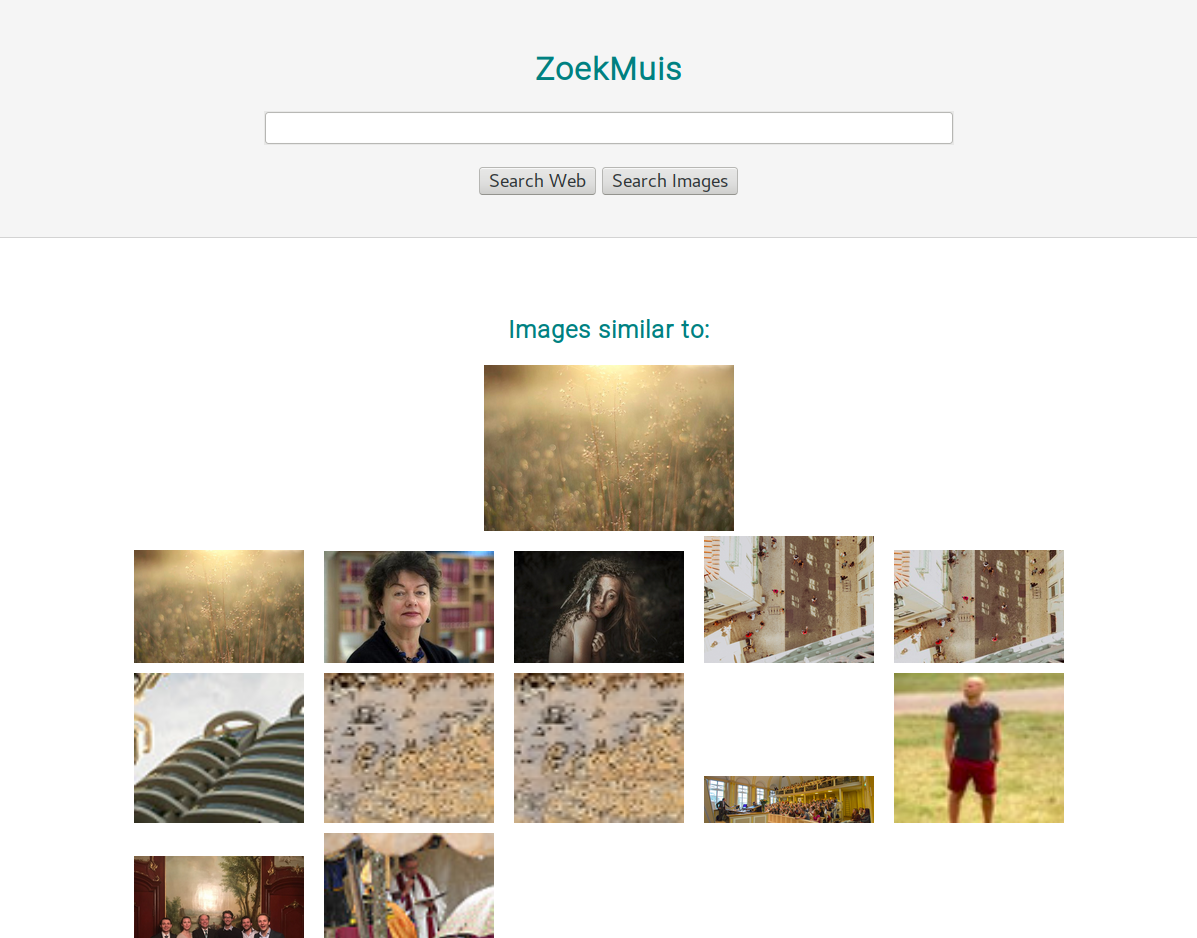
\includegraphics[width=12cm]{zoekmuis_color.png}\newline
Another image query\newline

\includegraphics[width=12cm]{zoekmuis_images2.png}\newline


\end{document}
